\documentclass[aspectratio=169]{beamer}

\usetheme{Frankfurt}
\setbeamercolor{section in head/foot}{bg=lightgray}
\setbeamertemplate{footline}[frame number]
\beamertemplatenavigationsymbolsempty
\usepackage{appendixnumberbeamer}

\usefonttheme{professionalfonts}
\usepackage{graphicx}
\usepackage{booktabs}\usepackage{array}
\usepackage{amsmath}
\usepackage{tikz}
\usetikzlibrary{positioning,arrows.meta,calc}
\usepackage{hyperref}
\hypersetup{colorlinks=true, urlcolor=blue, linkcolor=blue, citecolor=blue}

\definecolor{gtnavy}{HTML}{003057}
\definecolor{gtgold}{HTML}{B3A369}
\definecolor{gtred}{HTML}{8B0000}
\newcommand{\lead}[1]{{\small\itshape\textcolor{gtnavy!80}{#1}}\par\vspace{1.5mm}}

\newcommand{\bi}{\begin{itemize}}
\newcommand{\ei}{\end{itemize}}
\newcommand{\m}{\item}
\newcommand{\be}{\begin{enumerate}}
\newcommand{\ee}{\end{enumerate}}
\newcommand{\ul}{\underline}

\title[Why Hasn't Crypto Taken Over?]{\LARGE{What Is Crypto?} \\
\vspace{1mm}
\large{Why Hasn't It Taken Over? And Will AI Change That?} \\
\vspace{3mm}
\small{HBS AMP210 Reunion, Istanbul}}
\author[Joseph Hall and Brian Hall]{Joseph Hall and Brian Hall}
\institute[GT and HBS]{Georgia Institute of Technology and Harvard Business School}
\date{October 23, 2026}



\begin{document}

\begin{frame}[label=main-title]
\titlepage
\vspace{-27mm}
\begin{flushright}
\begin{tabular}{@{}c@{}}

\includegraphics[height=2.0cm]{fig_qr_site.png}\\[0.4mm]
{\scriptsize josephphall.com}
\end{tabular}\hspace{1mm}
\end{flushright}
\end{frame}

%=====================================================================
\section{The Question}
%=====================================================================

\begin{frame}[label=main-poll]
\frametitle{How Far Will You Let AI Agents Handle Your Money?}

\vfill
\begin{center}
{\large Has an AI ever bought something or moved money for you?\\ How did it go?}\\[10mm]
{\large In five years, what will you let an AI buy\\ with no one approving each payment?}
\end{center}
\vfill
\end{frame}


\begin{frame}[label=main-stakes]
\frametitle{An Agent Spending \$10,000 for You Raises Three Questions}

Would you let an AI spend \$10,000 of your family's money furnishing a new living room and kitchen this week, from any seller online, with no one approving each payment?
\vspace{4mm}

The agent must deal with sellers it cannot trust, and who cannot trust it. Every deal raises three questions.
\be
\m Will this agent obey the rules set for it?
\m Who is the other agent? Does it hold the value it claims, and can it transfer it?
\m Will it keep its promises?
\ee
\end{frame}


\begin{frame}[label=main-thesis]
\frametitle{Blockchains Fill a Pressing Need in an Economy of AI Agents}

\bi
\m Blockchains, shared ledgers (records of who owns what) that no one controls, enforce rules and track identity, value, and promises in code fully legible to AI agents
\m Crypto is the money recorded on a blockchain
\m A smart contract is a program on a blockchain that keeps a promise
\ei
\vspace{6mm}
\begin{center}
{\large\textcolor{gtnavy}{\textbf{If humans had not already created crypto and smart contracts,\\ AI agents would have needed to create them on their own}}}
\end{center}
\par\vspace{0pt plus 1fill}\hfill{\scriptsize \hyperlink{appx-agentsnow}{\beamergotobutton{Agents on chain today}}}
\end{frame}


%=====================================================================
\section{Telling an AI the Rules}
%=====================================================================
\begin{frame}[label=main-preview]
\frametitle{Four Questions Lead from Bitcoin to an Economy of AI Agents}

\vfill
{\large
\be
\setlength{\itemsep}{3mm}
\m In order to trust an AI with our money, why can't we just tell it the rules?
\m How can money work with no trust, and no one able to stop it?
\m How did Ethereum make promises enforce themselves? \textcolor{gray}{\normalsize (the case you read)}
\m Why hasn't crypto taken over?\\ \hspace*{6mm}$\bullet$\ Will AI change that fact?
\ee}
\vfill
\end{frame}


\begin{frame}[label=main-rule]
\frametitle{A Rule in a Smart Contract Holds Where a Rule in an AI Prompt Can Slip}
\lead{Rules. Will an agent obey the rules set for it?}

\begin{center}
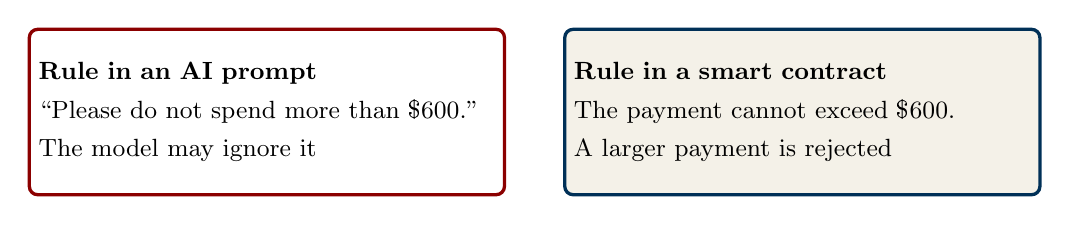
\begin{tikzpicture}[b/.style={draw, very thick, rounded corners=3pt, text width=5.8cm, minimum height=2.1cm, align=left, font=\small}]
\node[b, draw=gtred] (p) at (0,0) {\textbf{Rule in an AI prompt}\\[1mm] ``Please do not spend more than \$600.''\\[1mm] The model may ignore it};
\node[b, draw=gtnavy, fill=gtgold!15] (s) at (6.8,0) {\textbf{Rule in a smart contract}\\[1mm] The payment cannot exceed \$600.\\[1mm] A larger payment is rejected};
\end{tikzpicture}
\end{center}

\bi
\m Crypto rules cannot be broken by any one party, and anyone can verify them in advance, so another agent can check them before it deals
\m The agent wears handcuffs, and everyone on the street can prove it holds no key
\m Bitcoin was the first such system, built for money; Ethereum added smart contracts
\ei
\par\vspace{0pt plus 1fill}\hfill{\scriptsize \hyperlink{appx-harness}{\beamergotobutton{The harness}}}
\end{frame}


\begin{frame}[label=main-opposite]
\frametitle{AI and Blockchains Have Almost Opposite Strengths}
\lead{Rules. What does a blockchain add to an AI agent?}

\begin{columns}[T]
\column{0.47\textwidth}
\textbf{\textcolor{gtnavy}{AI}}
\bi
\m Explores a wide range of possibilities and works behind the scenes in unpredictable ways
\m The unpredictability is the value! You ask because you don't already know
\ei
\column{0.47\textwidth}
\textbf{\textcolor{gtnavy}{Blockchain}}
\bi
\m Everything is set in stone and verifiable
\m It works the way it claims, and you can see for yourself
\ei
\end{columns}
\vspace{4mm}
Both need a digital world. Bitcoin launched in 2009, Ethereum, the first blockchain for smart contracts, in 2015, and ChatGPT in 2022.
\end{frame}


%=====================================================================
\section{What Bitcoin Invented}
%=====================================================================
\begin{frame}
\vfill
\begin{itemize}
\setlength{\itemsep}{3mm}
\item[] \textcolor{gray}{In order to trust an AI with our money, why can't we just tell it the rules?}
\item[\textcolor{gtnavy}{$\blacktriangleright$}] {\large\textcolor{gtnavy}{\textbf{How can money work with no trust, and no one able to stop it?}}}
\item[] \textcolor{gray}{How did Ethereum make promises enforce themselves?}
\item[] \textcolor{gray}{Why hasn't crypto taken over?}
\item[] \textcolor{gray}{\hspace*{8mm}Will AI change that fact?}
\end{itemize}
\vfill
\end{frame}


\begin{frame}[label=main-bitcoin]
\frametitle{Bitcoin Makes Money Scarce Without Anyone in Charge}
\lead{Value. How can money stay scarce with no one in charge?}

\bi
\m Money replaces barter. It must be scarce, and everyone must be able to verify that it is scarce
\m Gold is scarce by nature. A king's coin is scarce because only the king owns the stamp, and counterfeiters were executed
\m Satoshi Nakamoto (2008) made money scarce by math. Whoever solves a hard puzzle is king for one round: a mathocracy
\m Satoshi's wallet holds about \$90 billion of bitcoin, untouched since it was mined in 2009 and 2010
\m James Howells's 8,000 bitcoin, about \$660 million, are out of reach. In 2013 he threw out the hard drive holding the key, and it lies in a Welsh landfill
\ei
\vfill
{\scriptsize Satoshi's identity is unknown. Researchers attribute about 1.1 million bitcoin to Satoshi, valued at \$81,952 per bitcoin (mempool.space, October 22, 2026). In principle, Satoshi could have been an AI.}
\par\vspace{0pt plus 1fill}\hfill{\scriptsize \hyperlink{appx-copies}{\beamergotobutton{25,000 copies}}}
\end{frame}


\begin{frame}[label=main-metaphor]
\frametitle{One Metaphor Runs from Messages to Money to Smart Contracts}
\lead{Identity, value, promises. How do the pieces fit together?}

{\small\textcolor{gtred}{\textbf{METAPHOR}}}\par\vspace{2mm}
\renewcommand{\arraystretch}{1.6}
\begin{tabular}{@{}>{\raggedright\arraybackslash}p{0.25\textwidth}>{\raggedright\arraybackslash}p{0.52\textwidth}>{\raggedright\arraybackslash}p{0.17\textwidth}@{}}
\textbf{\textcolor{gtnavy}{1. Masks speak messages}} & You are a secret key hiding behind a mask. Anyone can prove the one wearing the mask created the message & \textbf{Digital signatures} \\
\textbf{\textcolor{gtnavy}{2. Messages are woven into ``songs'' to create money}} & Creating a new rhyme is hard, which keeps money scarce. The rhymes have to endure, which keeps money secure & \textbf{Bitcoin} \\
\textbf{\textcolor{gtnavy}{3. A richer grammar allows smart contracts}} & A verse can now say ``Send money from A to B only if X, Y, and Z'' & \textbf{Ethereum} \\
\end{tabular}
\par\vspace{0pt plus 1fill}\hfill{\scriptsize \hyperlink{appx-signature}{\beamergotobutton{Masks and messages}} \hyperlink{appx-key}{\beamergotobutton{The private key}} \hyperlink{appx-sigformal}{\beamergotobutton{Signatures, formally}} \hyperlink{appx-cyberweek}{\beamergotobutton{This week in cybersecurity}}}
\end{frame}


\begin{frame}[label=main-verse]
\frametitle{From Messages to Money}
\lead{Value. With no one in charge, how does everyone agree on one copy of the ledger?}

\textcolor{gtred}{\textbf{METAPHOR}}: the ledger is a song, and messages become money when they are woven into it. Each new verse, a \textbf{block}, says three things.
\be
\m ``I remember everything that came before''
\m ``Here are new payments''
\m ``I won a costly guessing contest, so I get to add a verse''
\ee

\bi
\m Checking a rhyme is easy; writing one is hard. The writer, a \textbf{miner}, earns new bitcoin
\m Safety in the system, the guarantee you cannot \textbf{double-spend} (spend the same coin twice), comes from the fact that if you change an old verse, the new ones stop rhyming
\ei
\par\vspace{0pt plus 1fill}\hfill{\scriptsize \hyperlink{appx-hash}{\beamergotobutton{Hashes}} \hyperlink{appx-puzzle}{\beamergotobutton{The puzzle}} \hyperlink{appx-merkle}{\beamergotobutton{Merkle trees}} \hyperlink{appx-supply}{\beamergotobutton{21 million cap}} \hyperlink{appx-longest}{\beamergotobutton{Longest chain}} \hyperlink{appx-majority}{\beamergotobutton{Majority attack}}}
\end{frame}


\begin{frame}[label=main-difficulty]
\frametitle{Mining Bitcoin Is About 130 Trillion Times Harder Than in 2009}

\begin{center}
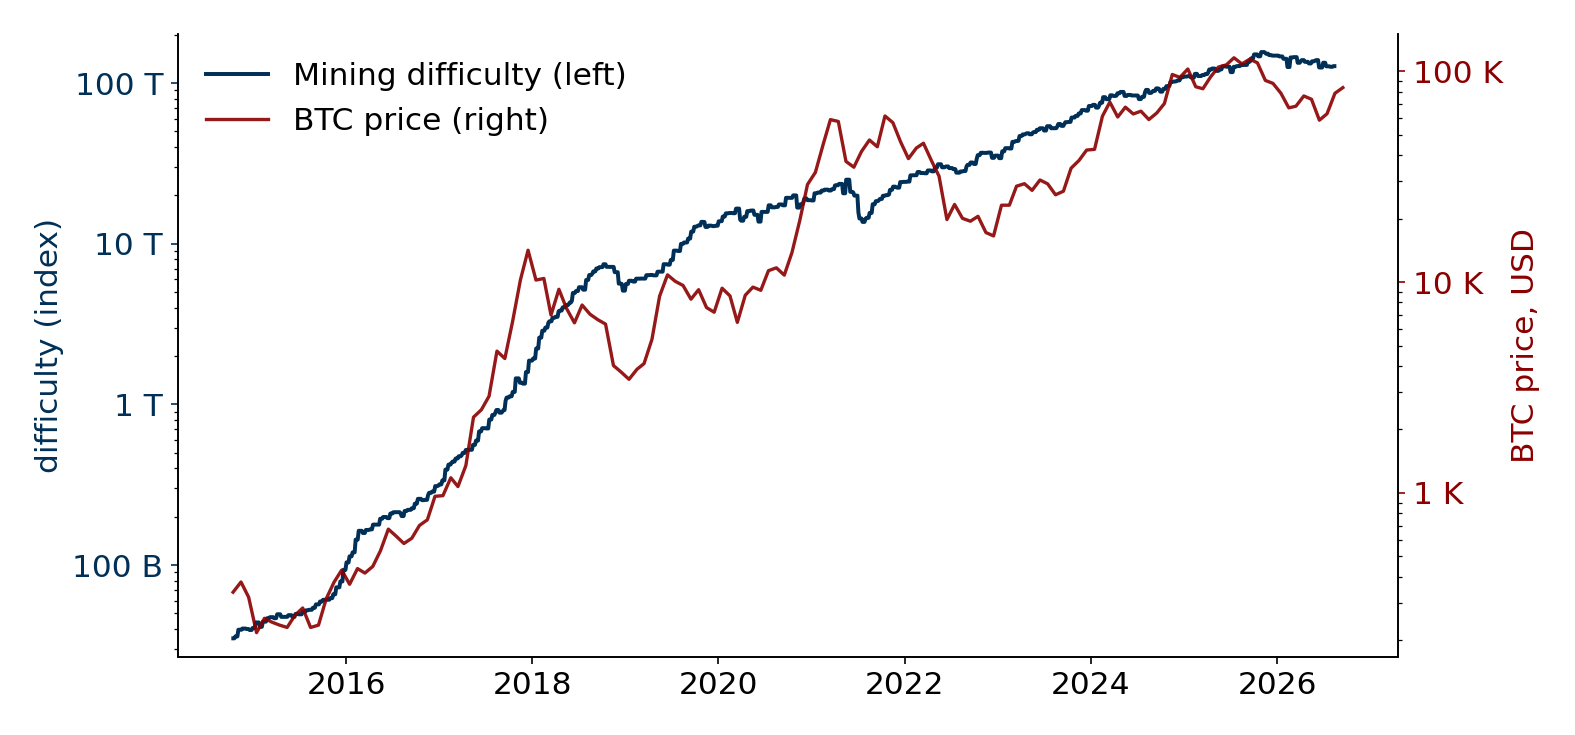
\includegraphics[width=.56\textwidth]{fig_btc_difficulty.png}
\end{center}
\vspace{1mm}
{\scriptsize Difficulty (left) and the bitcoin price (right) rise together. Difficulty, how hard the contest is, is an index, 1 = the first block (January 2009). Log scales. Sources: Blockchain.com (difficulty), Yahoo Finance (monthly BTC-USD close), September 2026.}
\par\vspace{0pt plus 1fill}\hfill{\scriptsize \hyperlink{appx-moneypot}{\beamergotobutton{Money-pot game}} \hyperlink{appx-potlesson}{\beamergotobutton{Money-pot lesson}} \hyperlink{appx-zeros}{\beamergotobutton{Leading zeros}}}
\end{frame}


\begin{frame}[label=main-energy]
\frametitle{Bitcoin Uses About a Third as Much Electricity as Data Centers}
\lead{Value. What does the contest cost, and what does that buy?}

\begin{center}
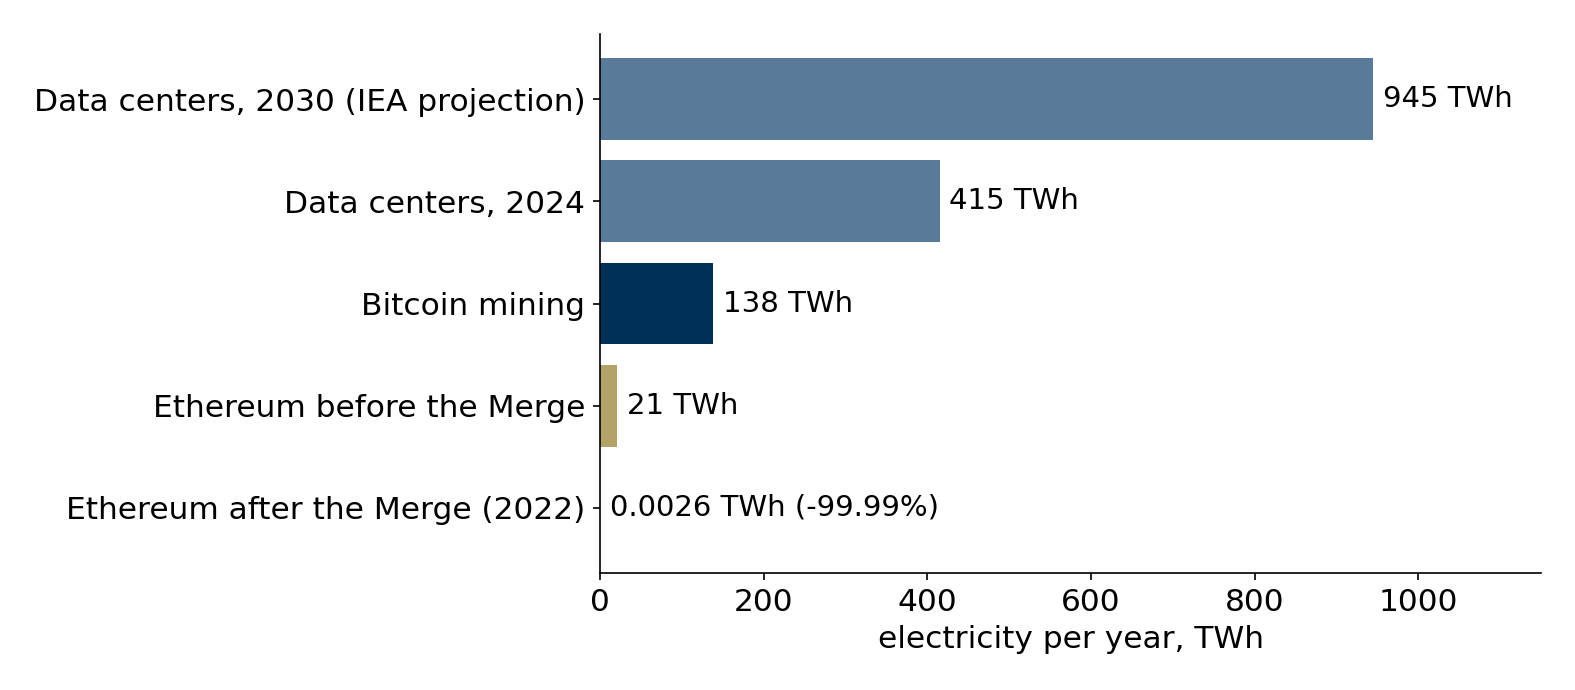
\includegraphics[width=.46\textwidth]{fig_energy.png}
\end{center}
\vspace{-2mm}
{\small Bitcoin uses about 0.4\% of world electricity, and data centers about 1\%. Bitcoin spends electricity on purpose, which keeps new coins scarce and its history costly to fake. In 2022 Ethereum, the next section's network, switched to \textbf{proof of stake}: those who add blocks post its currency as a bond, and its electricity use fell by about 99.99\%.}

\vspace{1mm}
{\scriptsize Sources: Cambridge Digital Mining Industry Report (2025); IEA, \emph{Energy and AI} (2025); Ember (30,856 TWh in 2024); Synergy Research (2025); ethereum.org.}
\par\vspace{0pt plus 1fill}\hfill{\scriptsize \hyperlink{appx-lights}{\beamergotobutton{Lights at night}}}
\end{frame}


\begin{frame}[label=main-btcrecap]
\frametitle{Bitcoin Gives an Agent Identity and Value, and Leaves Two Gaps}

\textbf{\textcolor{gtnavy}{What Bitcoin gives an agent}}
\bi
\m \textbf{Identity}: a key only its holder can sign and spend with
\m \textbf{Value}: a balance anyone can verify, on a history too costly to rewrite
\ei
\vspace{1mm}
\textbf{\textcolor{gtred}{What Bitcoin lacks}}
\bi
\m \textbf{Speed}: about 5 transactions per second, against about 8,000 for Visa. Faster networks now run on top of the main chains
\bi
\m To a user, a payment waits about 10 minutes and pays a flat fee of about 12 cents, whatever the amount sent
\ei
\m \textbf{Promises}: a Bitcoin verse mostly says ``send 1 bitcoin to Brian.'' Ethereum, the next section, gives verses a richer grammar
\ei
\vfill
{\scriptsize Average use, October 2024 to September 2025: Bitcoin 161.5 million confirmed transactions (Blockchain.com); Visa 257.5 billion on its networks (Visa fiscal 2025 10-K). Fee for a typical 141-byte payment at the going rate, with bitcoin at \$81,936 (mempool.space, October 19, 2026).}
\end{frame}


%=====================================================================
\section{What Ethereum Added}
%=====================================================================
\begin{frame}
\vfill
\begin{itemize}
\setlength{\itemsep}{3mm}
\item[] \textcolor{gray}{In order to trust an AI with our money, why can't we just tell it the rules?}
\item[] \textcolor{gray}{How can money work with no trust, and no one able to stop it?}
\item[\textcolor{gtnavy}{$\blacktriangleright$}] {\large\textcolor{gtnavy}{\textbf{How did Ethereum make promises enforce themselves?}}}
\item[] \textcolor{gray}{Why hasn't crypto taken over?}
\item[] \textcolor{gray}{\hspace*{8mm}Will AI change that fact?}
\end{itemize}
\vfill
\end{frame}


\begin{frame}[label=main-ethereum]
\frametitle{Ethereum Gives the Verses a Richer Grammar}
\lead{Promises. How can a promise enforce itself?}

\bi
\m A Bitcoin verse says ``send money from A to B.'' An Ethereum verse can say ``send money from A to B only if X, Y, and Z.'' Its currency is \textbf{ether}
\m A \textbf{smart contract} is such a verse: ``here is a new account, and it obeys these rules''
\m Its rules are public code, so any agent can read exactly what it will do
\m A smart contract can also create a \textbf{token}, a digital asset such as a voting share or a digital dollar
\ei
\end{frame}


\begin{frame}[label=main-escrow]
\frametitle{An Escrow Contract Binds a Machine as Tightly as a Person}
\lead{Promises. What does a smart contract look like at work?}

\begin{center}
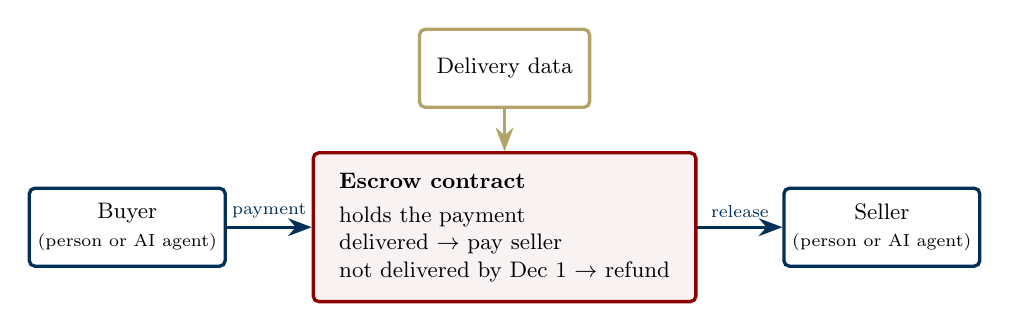
\begin{tikzpicture}[scale=0.9, transform shape,
  party/.style={draw=gtnavy, very thick, rounded corners=2pt, minimum width=2.4cm, minimum height=1.1cm, font=\small, align=center},
  code/.style={draw=gtred, very thick, fill=gtred!5, rounded corners=2pt, minimum width=5.4cm, minimum height=2.1cm, align=left, font=\small},
  arr/.style={-{Stealth[length=3mm]}, very thick, gtnavy}]
\node[code] (c) {\textbf{Escrow contract}\\[1mm] holds the payment\\ delivered $\rightarrow$ pay seller\\ not delivered by Dec 1 $\rightarrow$ refund};
\node[party, left=1.2cm of c] (b) {Buyer\\ {\scriptsize (person or AI agent)}};
\node[party, right=1.2cm of c] (s) {Seller\\ {\scriptsize (person or AI agent)}};
\node[party, above=0.6cm of c, draw=gtgold] (o) {Delivery data};
\draw[arr] (b) -- node[above, font=\scriptsize]{payment} (c);
\draw[arr] (c) -- node[above, font=\scriptsize]{release} (s);
\draw[arr, gtgold] (o) -- (c);
\end{tikzpicture}
\end{center}

\vspace{1mm}
For a couch, the seller can see that the money is there, and the buyer pays only if the couch arrives. The contract is only as good as the data that feeds it.
\end{frame}


\begin{frame}[label=main-twobytwo]
\frametitle{Simple Contracts That Serve a Real Need Work Today}
\lead{Promises. Which promises can code keep today?}

\begin{center}
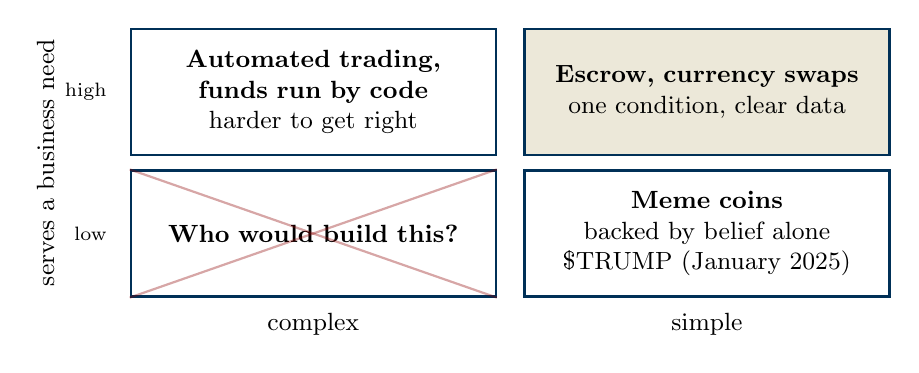
\begin{tikzpicture}[q/.style={draw=gtnavy, thick, text width=4.4cm, minimum height=1.6cm, align=center, font=\small}]
\node[q] at (0,1.8) {\textbf{Automated trading,}\\ \textbf{funds run by code}\\ harder to get right};
\node[q, fill=gtgold!25] at (5.0,1.8) {\textbf{Escrow, currency swaps}\\ one condition, clear data};
\node[q] (x) at (0,0) {\textbf{Who would build this?}};
\draw[gtred, thick, opacity=0.35] (x.south west) -- (x.north east); \draw[gtred, thick, opacity=0.35] (x.north west) -- (x.south east);
\node[q] at (5.0,0) {\textbf{Meme coins}\\ backed by belief alone\\ \$TRUMP (January 2025)};
\node[font=\scriptsize, anchor=east] at (-2.5,1.8) {high};
\node[font=\scriptsize, anchor=east] at (-2.5,0) {low};
\node[font=\small, rotate=90] at (-3.4,0.9) {serves a business need};
\node[font=\small] at (0,-1.15) {complex};
\node[font=\small] at (5.0,-1.15) {simple};
\end{tikzpicture}
\end{center}
\vspace{1mm}
An escrow could carry the \$10,000 from the opening question.
\end{frame}


\begin{frame}[label=main-dao]
\frametitle{The DAO Hack Forced Ethereum to Decide Whether Code Is Final}
\lead{Rules. What if the code itself has a flaw?}

{\small In June 2016 an attacker drained about \$83M of ether from \textbf{The DAO}, a venture fund run by code and token votes. Such organizations are called DAOs. A \textbf{hard fork} would override the code.}
\vspace{2mm}
\begin{center}
{\large Should Vitalik Buterin, Ethereum's creator, back the hard fork?\\[1mm] Is code law, or is cooperation law?}
\end{center}
\pause
\vspace{1mm}
\bi
\small
\m July 20, 2016: Ethereum forked, and investors got their ether back
\m Holdouts kept the old chain, Ethereum Classic, whose math still checks out
\m The community set a norm beyond any written code. If what you do is palpably unfair and exploitative, the community will coordinate to cut you out
\m Ethereum showed that it can and will rely on human judgment. Bitcoin is the purest version of money; Ethereum is a social project
\ei
\par\vspace{0pt plus 1fill}\hfill{\scriptsize \hyperlink{appx-org}{\beamergotobutton{Code and culture}}}
\end{frame}


%=====================================================================
\section{Why Crypto Stalled}
%=====================================================================
\begin{frame}
\vfill
\begin{itemize}
\setlength{\itemsep}{3mm}
\item[] \textcolor{gray}{In order to trust an AI with our money, why can't we just tell it the rules?}
\item[] \textcolor{gray}{How can money work with no trust, and no one able to stop it?}
\item[] \textcolor{gray}{How did Ethereum make promises enforce themselves?}
\item[\textcolor{gtnavy}{$\blacktriangleright$}] {\large\textcolor{gtnavy}{\textbf{Why hasn't crypto taken over?}}}
\item[] \textcolor{gray}{\hspace*{8mm}Will AI change that fact?}
\end{itemize}
\vfill
\end{frame}


\begin{frame}[label=main-prices]
\frametitle{Bitcoin Fell by Half and Ether by About 60\% from Their 2025 Highs}

\begin{center}
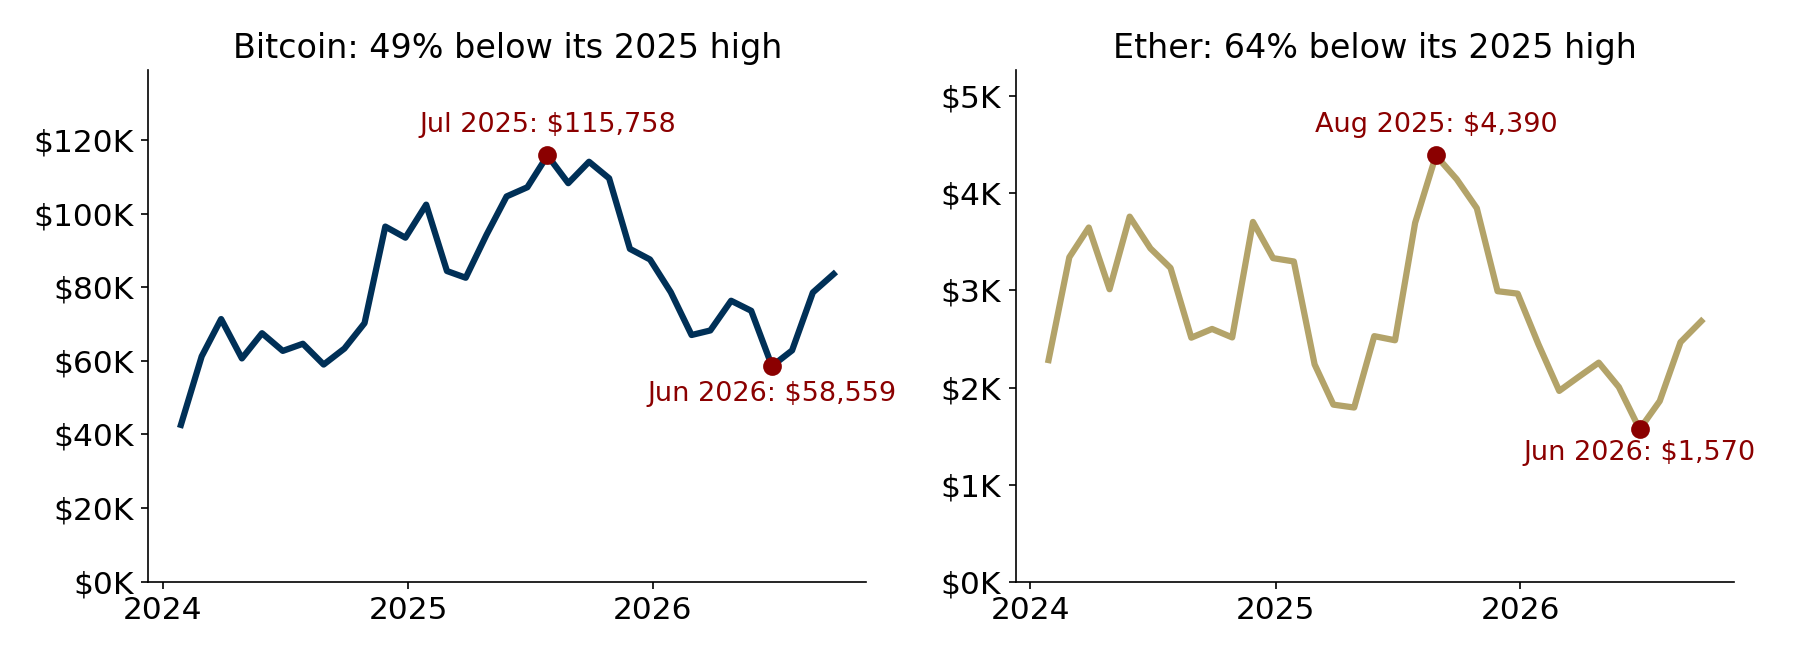
\includegraphics[width=.89\textwidth]{fig_crypto_prices.png}
\end{center}
\vspace{1mm}
Ethereum's community resolved The DAO, and crypto still has not taken off. Bitcoin remains about double its January 2024 price.
\vfill
{\scriptsize Monthly closing prices, U.S. dollars, to June 2026 lows (Yahoo Finance, October 2026). Bitcoin's January 2024 close \$42,583; September 2026 close \$83,554.}
\end{frame}


\begin{frame}[label=main-authority]
\frametitle{Authority Recreated the Technology First}
\lead{Why did crypto not replace the trusted keepers?}

\bi
\m It was easier for the authority to recreate the technology than for the technology to recreate the authority
\m Crypto has not leapt from a tool for nerds to a tool for the masses, whose experience has been getting defrauded
\m Coinbase rebuilt a trusted keeper from the crypto side, the opposite of FTX
\bi
\m FTX used customers' money to cover its trading firm's losses, and collapsed in 2022
\m Coinbase kept behaving as a trustworthy keeper. It joined the S\&P 500 in 2025, and in April 2026 won conditional approval for a federal trust bank charter
\ei
\ei
\vspace{1mm}
The biggest recent growth in blockchain use has not been ground-up growth\\
led by anonymous crypto pirates.\\[2mm]
It has been trusted financial intermediaries\\
adopting digital signatures and smart contracts.
\par\vspace{0pt plus 1fill}\hfill{\scriptsize \hyperlink{appx-incumbents}{\beamergotobutton{Incumbents}}}
\end{frame}


\begin{frame}[label=main-tokens]
\frametitle{Tokens Differ in What Stands Behind Them}
\lead{Value. Which tokens hold their value, and who stands behind them?}

\begin{center}
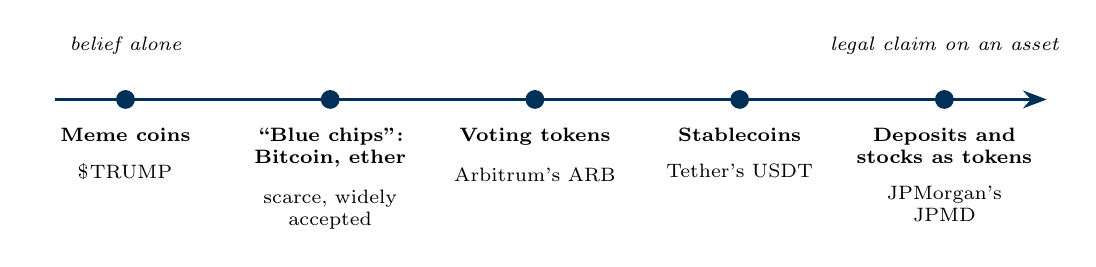
\begin{tikzpicture}[
  st/.style={align=center, font=\scriptsize, text width=2.25cm},
  dot/.style={circle, fill=gtnavy, inner sep=2.4pt}]
\draw[-{Stealth[length=3mm]}, very thick, gtnavy] (0,0) -- (12.6,0);
\node[font=\scriptsize\itshape, above=10pt] at (0.9,0.1) {belief alone};
\node[font=\scriptsize\itshape, above=10pt] at (11.3,0.1) {legal claim on an asset};
\foreach \x/\h/\t [count=\i] in {0.9/{Meme coins}/{\$TRUMP},
                      3.5/{``Blue chips'': Bitcoin, ether}/{scarce, widely accepted},
                      6.1/{Voting tokens}/{Arbitrum's ARB},
                      8.7/{Stablecoins}/{Tether's USDT},
                      11.3/{Deposits and stocks as tokens}/{JPMorgan's JPMD}} {
  \node[dot] at (\x,0) {};
  \node[font=\scriptsize\bfseries, below=4pt, text width=2.25cm, align=center] (lab\i) at (\x,-0.1) {\h};
  \node[st, below=1pt of lab\i] {\t};
}
\end{tikzpicture}
\end{center}
\bi
\m A \textbf{stablecoin} is a token pegged to a currency
\m The tokens closest to money depend on a trusted issuer
\ei
\end{frame}


\begin{frame}[label=main-stablecoin]
\frametitle{A Stablecoin Issuer Operates a Bank-Like Balance Sheet}
\lead{What stands behind a dollar token?}

\begin{columns}
\column{0.5\textwidth}
\centering
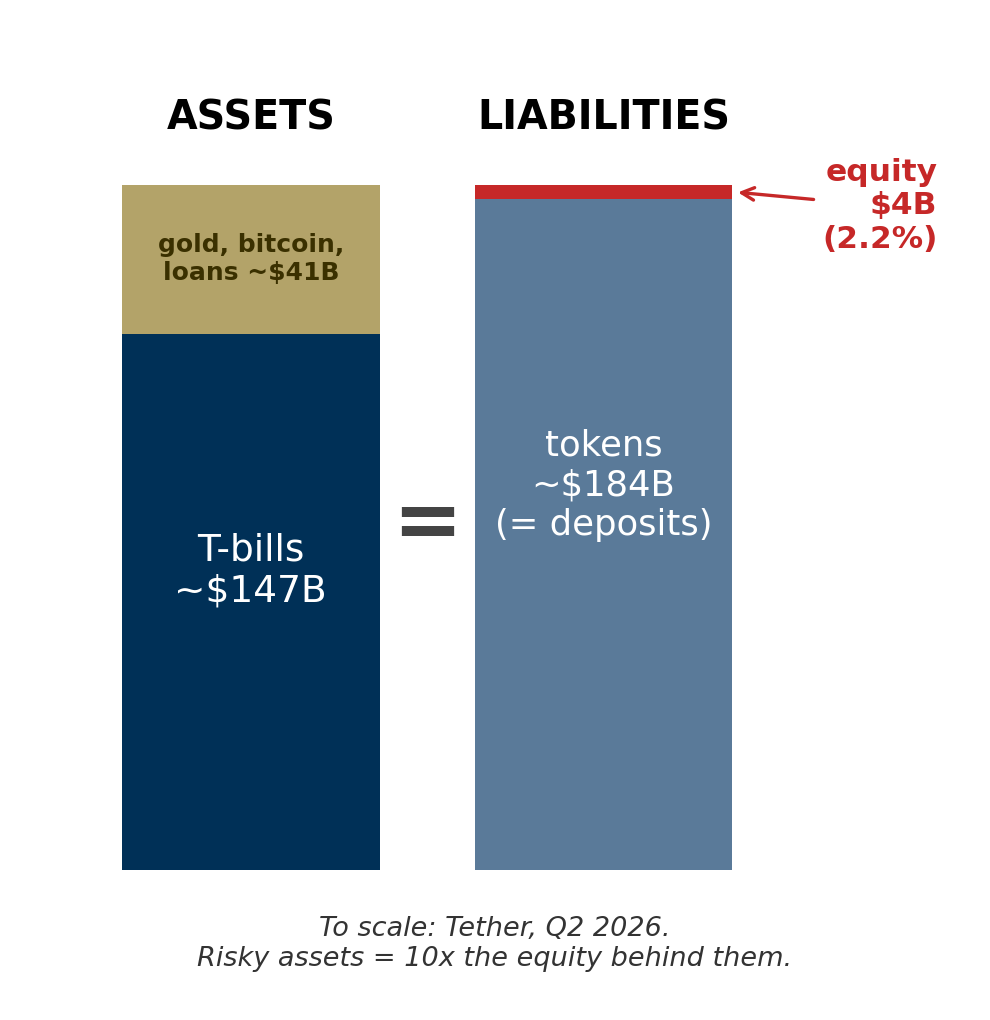
\includegraphics[height=0.74\textheight]{fig_issuer_balance_sheet.png}
\column{0.48\textwidth}
\footnotesize
\bi
\m Tether's tokens are its deposits, and its reserves are its assets (BDO, Q2 2026)
\m Equity is 2.2\% of assets, leverage of about 45 to 1
\m U.S. banks hold equity of 10\% of assets (FDIC, Q4 2025)
\ei
\vspace{4mm}
{\textcolor{gtnavy}{\textbf{The biggest cryptocurrency by volume today, the Tether USD Stablecoin (USDT) is backed by 1/5 the capital of a bank deposit}}}
\end{columns}
\par\vspace{0pt plus 1fill}\hfill{\scriptsize \hyperlink{appx-genius}{\beamergotobutton{GENIUS Act sources}}}
\end{frame}


\begin{frame}[label=main-problems]
\frametitle{Four Problems Drove Value Away from Honest Builders}
\lead{What drove users and honest builders away?}

\be
\m \textbf{Predators thrive}: transfers are irreversible, with no chargebacks or deposit insurance
\m \textbf{Builders cannot capture the value they create}, so schemes outcompete real projects
\m \textbf{App owners claim the value}, because users won't touch the chain directly
\m \textbf{Honest builders leave}
\ee
\vfill
{\scriptsize My assessment, developed in ``Economic Applications of Cryptography'' (Georgia Tech, 2026).}
\par\vspace{0pt plus 1fill}\hfill{\scriptsize \hyperlink{appx-fiveforces}{\beamergotobutton{Five forces}}}
\end{frame}


%=====================================================================
\section{What AI Changes}
%=====================================================================
\begin{frame}
\vfill
\begin{itemize}
\setlength{\itemsep}{3mm}
\item[] \textcolor{gray}{In order to trust an AI with our money, why can't we just tell it the rules?}
\item[] \textcolor{gray}{How can money work with no trust, and no one able to stop it?}
\item[] \textcolor{gray}{How did Ethereum make promises enforce themselves?}
\item[] \textcolor{gray}{Why hasn't crypto taken over?}
\item[] {\large\textcolor{gtnavy}{\hspace*{8mm}$\blacktriangleright$\ \textbf{Will AI change that fact?}}}
\end{itemize}
\vfill
\end{frame}


\begin{frame}[label=main-edges]
\frametitle{AI Is a Double-Edged Sword for Crypto}

\begin{columns}[T]
\column{0.47\textwidth}
\textbf{\textcolor{gtnavy}{The good edge}}
\bi
\m Agents need rules they cannot rewrite, which smart contracts supply
\m AI can handle crypto's complexity and surface only what the user needs
\ei
\column{0.47\textwidth}

\textbf{\textcolor{gtred}{The bad edge}}
\bi
\m Crypto communities decide through anonymous debate, once proof of human work
\m AI now writes like a person, so that proof is gone
\ei
\end{columns}
\end{frame}


\begin{frame}[label=main-rails]
\frametitle{Payment Networks Are Building Rails for AI Agents}
\lead{Good edge. Will agents pay through crypto?}

{\small Payment \textbf{rails} move money, as card networks do.}

\begin{center}
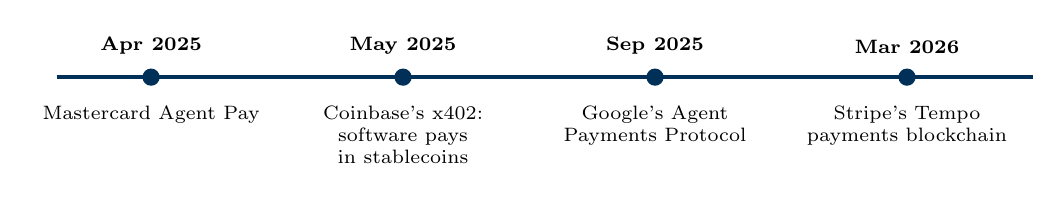
\begin{tikzpicture}[
  ev/.style={align=center, font=\scriptsize, text width=2.9cm},
  dot/.style={circle, fill=gtnavy, inner sep=2.2pt}]
\draw[very thick, gtnavy] (0,0) -- (12.4,0);
\foreach \x/\d/\t in {1.2/{Apr 2025}/{Mastercard Agent Pay},
                      4.4/{May 2025}/{Coinbase's x402: software pays in stablecoins},
                      7.6/{Sep 2025}/{Google's Agent Payments Protocol},
                      10.8/{Mar 2026}/{Stripe's Tempo payments blockchain}} {
  \node[dot] at (\x,0) {};
  \node[font=\scriptsize\bfseries, above=2pt] at (\x,0.1) {\d};
  \node[ev, below=4pt] at (\x,-0.1) {\t};
}
\end{tikzpicture}
\end{center}

\vspace{1mm}
x402 carried 75 million payments worth \$24 million in 30 days (September 2026).
\end{frame}


\begin{frame}[label=main-experiment]
\frametitle{An AI Agent Bought a Rangefinder with Stablecoins}
\lead{Good edge. What happened when we tried it?}

\begin{center}
\small
\begin{tabular}{>{\raggedright\arraybackslash}p{0.2\textwidth} >{\raggedright\arraybackslash}p{0.14\textwidth} >{\raggedright\arraybackslash}p{0.56\textwidth}}
\toprule
\textbf{Step} & \textbf{Elapsed} & \textbf{What a human had to do} \\
\midrule
Setup, once & 28 min & Fund the wallet, after two failed tries \\
This purchase & 15 min & Address, phone, one command, gift-card number \\
Next purchase & about 5 min & Gift-card number \\
\bottomrule
\end{tabular}
\end{center}

\bi
\m Paying took 2 seconds, with no fee: 92 USDC, a dollar stablecoin, for a gift card
\m The delays came from banks, checkouts built for people, and Anthropic's rules for Claude, which held even against a written mandate
\m \textbf{For ``buy me a rangefinder'' to suffice, merchants must take stablecoins and a signed mandate, the owner's limits, and AI developers' rules must honor it}
\ei
\vfill
{\scriptsize October 19, 2026. Bitrefill agent checkout (x402) on Base, transaction 0x22e6\ldots8c34 (basescan.org).}
\par\vspace{0pt plus 1fill}\hfill{\scriptsize \hyperlink{appx-mandate}{\beamergotobutton{Signed mandates}}}
\end{frame}


\begin{frame}[label=main-local]
\frametitle{A Local AI Could Handle Crypto's Complexity Without a Middleman}
\lead{Good edge. Can AI cut out the app owner?}

\bi
\m An \textbf{open-weight} model is an AI which can be distributed, downloaded, and run locally \textbf{without} the creator controlling it after distribution
\m You can find open-weight models without rules like Claude's on handling money, which slowed our agent's purchase
\m Such a model could manage keys and pay on a plain instruction, ``send Brian \$100,'' with no trusted app in between
\m If people instead use AI from a few large providers that work with governments, I believe that in that case AI will strengthen today's banks and payment networks
\ei
\end{frame}


\begin{frame}[label=main-forum]
\frametitle{AI Writing Weakened a \$3.5 Billion DAO's Forum}
\lead{Bad edge. What happens to debate when AI writes like a person?}

\begin{center}
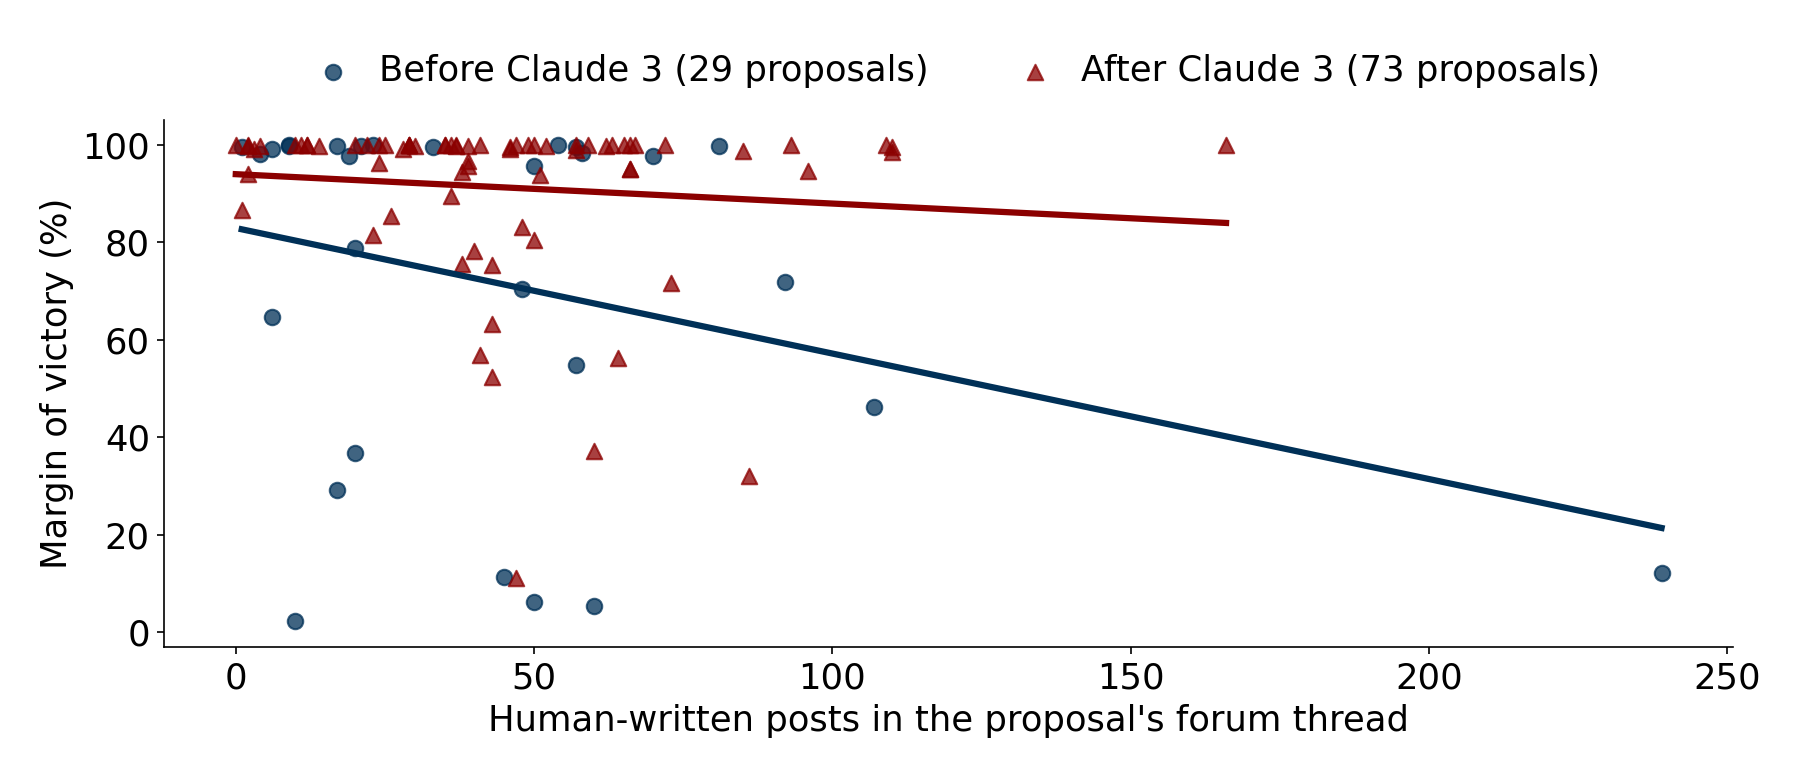
\includegraphics[width=.68\textwidth]{fig_forum_scatter.png}
\end{center}
\vspace{-1mm}
\bi
\small
\m More forum debate signaled a closer vote, until AI prose became indistinguishable
\m Anonymity, a design pillar of crypto, is the vulnerability
\ei
\vfill
{\scriptsize 102 Arbitrum DAO proposals; Claude 3 released March 4, 2024. Slope: $-0.26$ margin points per human post before, $-0.06$ after; structural-break test $p = 0.008$ (Huang and Hall, 2026).}
\end{frame}


\begin{frame}[label=main-second]
\frametitle{A Technology's Most Useful Application Often Arrives Second}
\lead{Why expect agents to become crypto's main users?}

\bi
\m Nuclear fission was first a weapon (1945). Its lasting use is about 9\% of world electricity (2025) \pause
\m Crypto's first application was money outside the state. Its more useful one is the smart contract
\m AI agents operating within coded limits are the most likely source of demand
\ei
\end{frame}


\begin{frame}[label=main-northstar]
\frametitle{If Humans Had Not Built Blockchains, AI Agents Would Have}

\bi
\m Keys, a shared ledger, and smart contracts let agents check identity, value, and promises without trusting each other
\m The \$10,000 can move through a contract that caps the spend and pays only on delivery
\m AI is a natural candidate to cut out the middleman and democratize crypto to unsophisticated people. That could be good, disastrous, or overhyped
\ei
\par\vspace{0pt plus 1fill}\hfill{\scriptsize \hyperlink{appx-synthesis}{\beamergotobutton{Strengths and weaknesses}} \hyperlink{appx-personhood}{\beamergotobutton{Personhood}} \hyperlink{appx-switchoff}{\beamergotobutton{Who can switch it off}}}
\end{frame}


\begin{frame}[label=main-discussion]
\frametitle{Discussion}

\bi
\m Will AI revive crypto's promise of money without a middleman, or strengthen the banks?
\m Which of your payments could an escrow contract handle, and what data would trigger them?
\m Would you let agents spend only through hard-capped contracts, knowing mistakes inside the cap cannot be reversed?
\ei
\end{frame}


\begin{frame}[label=main-credits]
\frametitle{Credits}

\begin{columns}
\column{0.72\textwidth}
\small
\bi
\m Bitcoin exposition partly adapted from teaching materials by \textbf{Anthony Lee Zhang}, with permission
\m Errors and opinions are mine alone
\ei
\column{0.24\textwidth}
\begin{center}

\includegraphics[width=\textwidth]{fig_qr_site.png}\\[0.5mm]
{\small josephphall.com}
\end{center}
\end{columns}
\par\vspace{0pt plus 1fill}\hfill{\scriptsize \hyperlink{appx-sources}{\beamergotobutton{Sources}}}
\end{frame}

%=====================================================================
\appendix
\section*{Appendix}
%=====================================================================

\begin{frame}
\vfill
\begin{center}
{\Huge\textcolor{gtnavy}{\textbf{Appendix}}}
\end{center}
\vfill
\end{frame}


\begin{frame}[label=appx-harness]
\frametitle{An AI Acts Only Through Its Harness}

\bi
\m The agent decides what to do. Its \textbf{harness} turns those decisions into actions
\m An agent that pays bills needs a harness that controls money
\ei
\par\vspace{0pt plus 1fill}\hfill{\scriptsize \hyperlink{main-rule}{\beamerreturnbutton{Back}}}
\end{frame}


\begin{frame}[label=appx-copies]
\frametitle{About 25,000 Computers Keep Identical Copies of the Ledger}

\bi
\m About 25,000 public computers keep and check the full history (Coin Dance, October 2026)
\m A forged entry disagrees with every other copy, so the network ignores it
\m No one owns all the machines, so no one can rewrite the record alone
\ei
\par\vspace{0pt plus 1fill}\hfill{\scriptsize \hyperlink{main-bitcoin}{\beamerreturnbutton{Back}}}
\end{frame}


\begin{frame}[label=appx-hash]
\frametitle{A Hash Is Instant to Check and Reversible Only by Guessing}

\bi
\m A \textbf{hash} turns any file into a short fingerprint (\href{https://emn178.github.io/online-tools/sha256.html}{live demo})
\m Same input, same fingerprint. Change one letter and the fingerprint changes completely
\m Checking takes an instant. Working backward takes guessing
\m Faking a matching fingerprint would take the whole Bitcoin network about 11 billion years
\ei
\vfill
{\scriptsize About $2^{128}$ guesses at the network's pace of 977 million trillion hashes per second (CoinWarz, September 29, 2026).}
\par\vspace{0pt plus 1fill}\hfill{\scriptsize \hyperlink{main-verse}{\beamerreturnbutton{Back}}}
\end{frame}


\begin{frame}[label=appx-puzzle]
\frametitle{The Puzzle Lets Strangers Agree on One History}

\bi
\m If adding a verse cost nothing, anyone could write endless competing histories
\m The \textbf{puzzle} (``proof of work'') is a lottery: computers guess until one finds a fingerprint with a rare pattern
\m Solving it takes machines and electricity, which cash can buy. A miner needs no special expertise, and AI lowers that bar further
\m Everyone follows the longest chain, because it proves the most work
\ei
\par\vspace{0pt plus 1fill}\hfill{\scriptsize \hyperlink{main-verse}{\beamerreturnbutton{Back}}}
\end{frame}


\begin{frame}[label=appx-merkle]
\frametitle{A Merkle Tree Checks One Verse Without Replaying the Whole Song}

\begin{columns}
\column{0.26\textwidth}
\centering
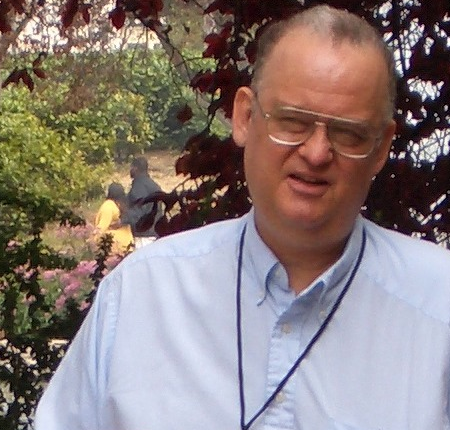
\includegraphics[width=\textwidth]{fig_ralph_merkle.jpg}\\[1mm]
{\scriptsize Ralph Merkle, Georgia Tech faculty 2003--2006}
\column{0.72\textwidth}
\bi
\m Merkle patented the hash tree in 1979 (U.S. Patent 4,309,569)
\m It confirms that one record belongs to a huge collection by checking a handful of fingerprints
\ei
\end{columns}
\par\vspace{0pt plus 1fill}\hfill{\scriptsize \hyperlink{main-verse}{\beamerreturnbutton{Back}}}
\end{frame}

\begin{frame}[label=appx-supply]
\frametitle{New Bitcoin Supply Halves Every Four Years, Toward a 21 Million Cap}

\begin{center}
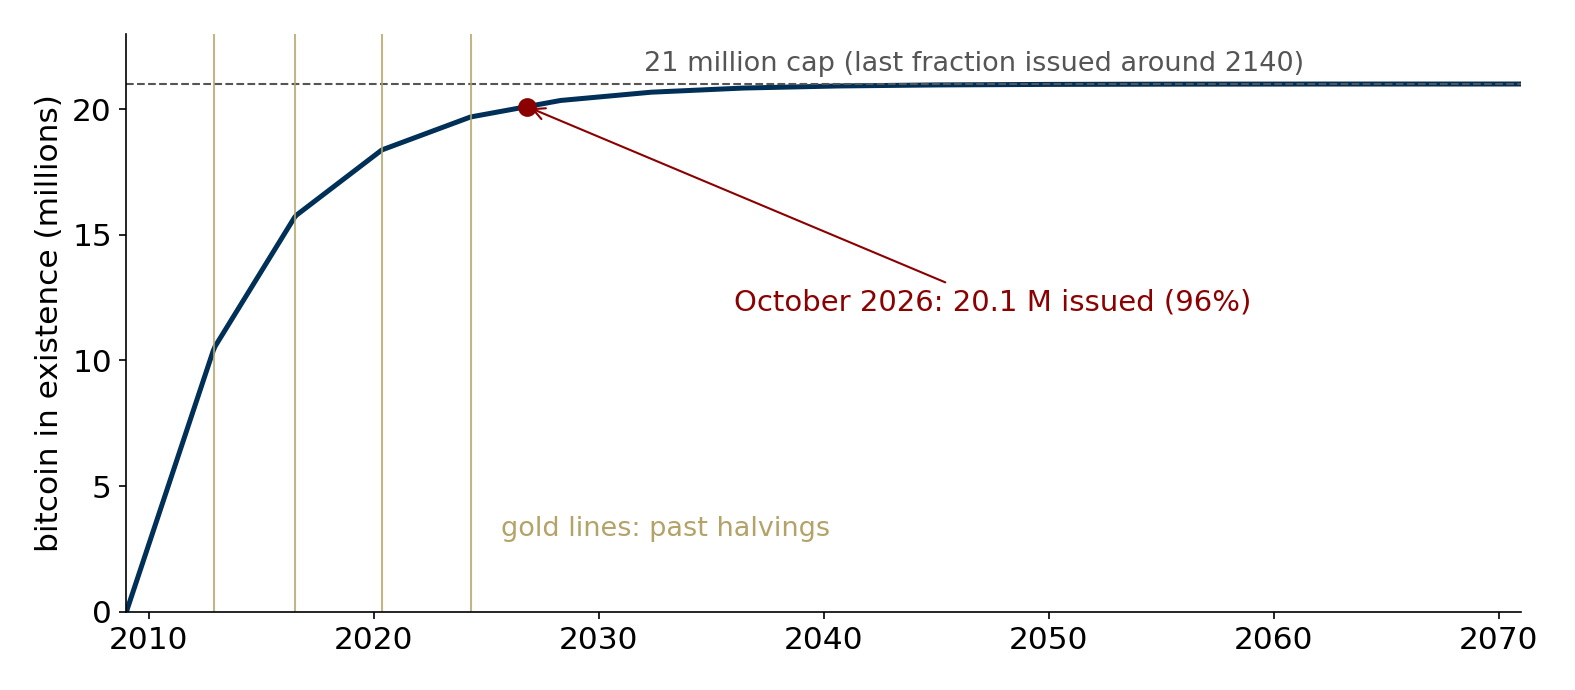
\includegraphics[width=.88\textwidth]{fig_btc_supply.png}
\end{center}

\scriptsize
Computed from Bitcoin's rules: the reward per block started at 50 bitcoin and halves every 210,000 blocks.

\par\vspace{0pt plus 1fill}\hfill{\scriptsize \hyperlink{main-verse}{\beamerreturnbutton{Back}}}
\end{frame}

\begin{frame}[label=appx-moneypot]
\frametitle{Take \$1 for Sure, or Share a \$10 Pot?}

\vfill
\begin{center}
{\Large Close your eyes and choose}
\end{center}
\vspace{4mm}
{\large
\be
\setlength{\itemsep}{4mm}
\m Receive \$1 for sure
\m Raise your hand to share a \$10 pot with everyone else who raises a hand
\ee}
\vfill
\par\vspace{0pt plus 1fill}\hfill{\scriptsize \hyperlink{main-difficulty}{\beamerreturnbutton{Back}}}
\end{frame}


\begin{frame}[label=appx-potlesson]
\frametitle{Miners Enter Until the Prize Is Competed Away}

\bi
\m With 11 hands, each gets about 91 cents. Entry stops at 10, when the pot pays exactly \$1
\m Everybody coordinates without speaking
\pause
\m Mining works the same way. Anyone with cash for machines and electricity can enter, until the profit is competed away
\ei
\par\vspace{0pt plus 1fill}\hfill{\scriptsize \hyperlink{main-difficulty}{\beamerreturnbutton{Back}}}
\end{frame}


\begin{frame}[label=appx-longest]
\frametitle{Everyone Follows the Longest Chain Because It Proves the Most Work}

\begin{quote}
``The longest chain not only serves as proof of the sequence of events witnessed, but proof that it came from the largest pool of CPU power.''
\hfill (Nakamoto, 2008)
\end{quote}

\bi
\m We follow the best builder: the longest chain shows who invested the most
\m A person, a firm, or an AI agent with a valid solution earns the bitcoin
\ei
\par\vspace{0pt plus 1fill}\hfill{\scriptsize \hyperlink{main-verse}{\beamerreturnbutton{Back}}}
\end{frame}

\begin{frame}[label=appx-majority]
\frametitle{A Majority of Computing Power Could Rewrite Recent History}

\bi
\m An attacker with more computing power than the rest of the network combined could build a longer chain in secret and release it
\m Everyone follows the longest chain, so the attacker's version would replace recent blocks
\m Nakamoto (2008) shows that the odds of an attacker with less than half the power catching up fall exponentially with each new block
\ei
\par\vspace{0pt plus 1fill}\hfill{\scriptsize \hyperlink{main-verse}{\beamerreturnbutton{Back}}}
\end{frame}
\begin{frame}[label=appx-zeros]
\frametitle{Writing the Next Verse Now Takes About 20 Leading Zeros}

\begin{center}
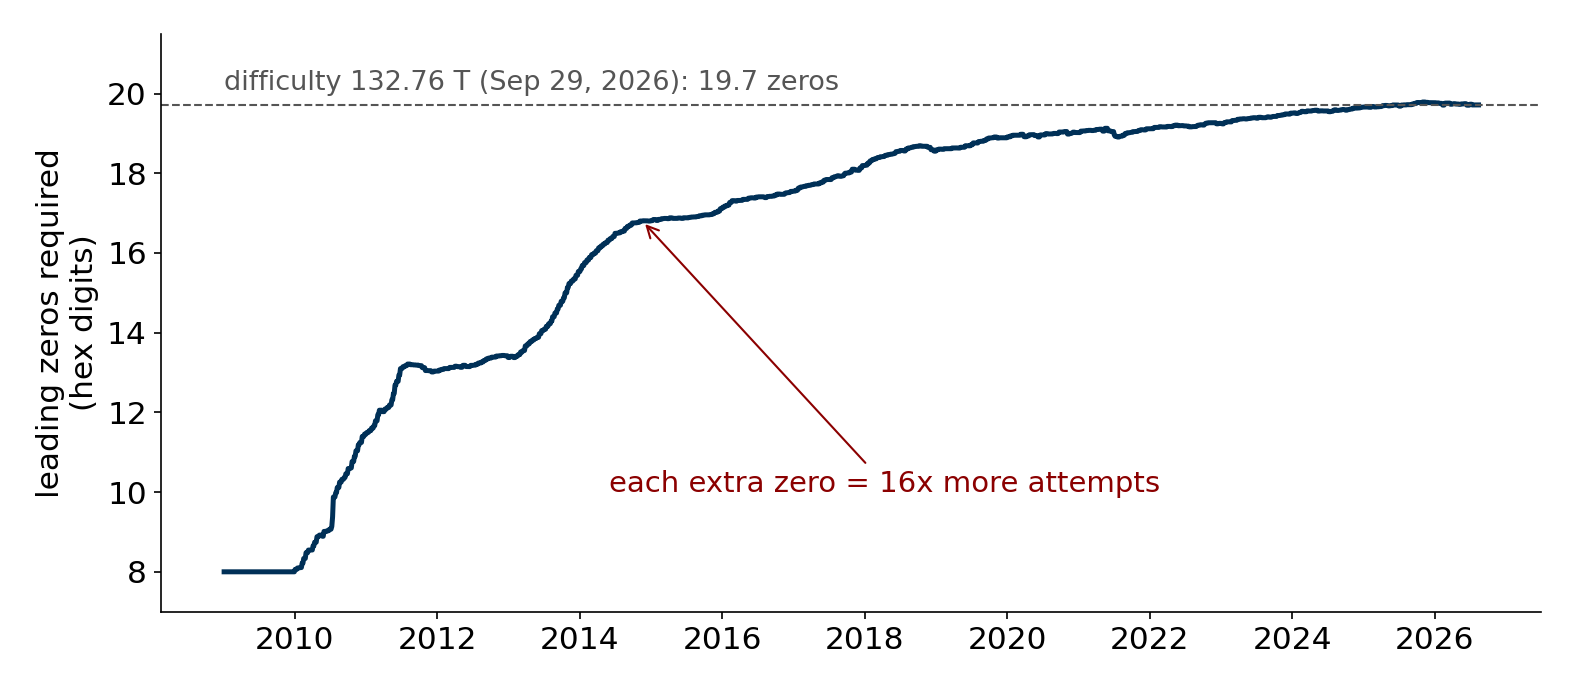
\includegraphics[width=.64\textwidth]{fig_leading_zeros.png}
\end{center}
{\small A winning guess must start with this many zeros. Each extra zero means 16 times more guesses.}\\[1mm]{\scriptsize Required zeros $= \log_{16}(\text{difficulty} \times 2^{32})$. Sources: Blockchain.com difficulty series; tip block hash from mempool.space, September 29, 2026.}
\par\vspace{0pt plus 1fill}\hfill{\scriptsize \hyperlink{main-difficulty}{\beamerreturnbutton{Back}}}
\end{frame}

\begin{frame}[label=appx-lights]
\frametitle{Burning Electricity Makes the History Costly to Fake}

\bi
\m Satellite images of lights at night show that autocracies overstate yearly GDP growth by about 35\% (Mart\'{i}nez, 2022) \pause
\m Bitcoin rests on the same idea. Real electricity spent makes the history costly to fake
\ei
\par\vspace{0pt plus 1fill}\hfill{\scriptsize \hyperlink{main-energy}{\beamerreturnbutton{Back}}}
\end{frame}

\begin{frame}[label=appx-genius]
\frametitle{Sources on the GENIUS Act and Foreign Issuers}

{\scriptsize
\bi
\setlength{\itemsep}{0pt}
\m \href{https://www.congress.gov/crs-product/IN12553}{Congressional Research Service, ``Stablecoin Legislation: An Overview of the GENIUS Act of 2025'' (IN12553)}
\m \href{https://www.congress.gov/bill/119th-congress/senate-bill/1582/text}{GENIUS Act, S.1582, 119th Congress (P.L. 119-27), statute text}
\m \href{https://www.law.cornell.edu/uscode/text/12/5902}{12 U.S.C. \S~5902, issuance and treatment of payment stablecoins}
\m \href{https://www.federalregister.gov/documents/2026/08/18/2026-16796/genius-act-regulations-on-payment-stablecoin-issuance-offer-and-sale}{Treasury, proposed rule on issuance, offer, and sale, \emph{Federal Register}, August 18, 2026}
\m \href{https://www.federalregister.gov/documents/2026/03/02/2026-04089/implementing-the-guiding-and-establishing-national-innovation-for-us-stablecoins-act-for-the}{Implementing the GENIUS Act, \emph{Federal Register}, March 2, 2026}
\m \href{https://www.occ.gov/news-issuances/bulletins/2026/bulletin-2026-3.html}{OCC Bulletin 2026-3, GENIUS Act notice of proposed rulemaking}
\m \href{https://www.chapman.com/publication-genius-act-rulemaking-tracker}{Chapman and Cutler, GENIUS Act rulemaking and reporting tracker}
\m \href{https://www.gibsondunn.com/the-genius-act-a-new-era-of-stablecoin-regulation/}{Gibson Dunn, ``The GENIUS Act: A New Era of Stablecoin Regulation''}
\m \href{https://www.yalejreg.com/nc/how-the-genius-act-regulates-foreign-issuersand-how-it-compares-to-europe-and-the-uk-by-benedikt-bartylla/}{Bartylla, ``How the GENIUS Act Regulates Foreign Issuers,'' \emph{Yale Journal on Regulation} (Notice \& Comment)}
\m \href{https://www.brookings.edu/articles/stablecoins-issues-for-regulators-as-they-implement-genius-act/}{Brookings, ``Stablecoins: Issues for Regulators as They Implement the GENIUS Act''}
\m \href{https://www.coindesk.com/news-analysis/2026/07/17/tether-s-usdt-hits-2-year-countdown-threatening-its-position-on-u-s-crypto-platforms}{CoinDesk, ``Tether's USDT Hits 2-Year Countdown,'' July 17, 2026}
\m \href{https://www.coindesk.com/news-analysis/2025/06/17/can-tether-s-dominance-survive-the-u-s-stablecoin-bill}{CoinDesk, ``Can Tether's Dominance Survive the U.S. Stablecoin Bill?'' June 17, 2025}
\m \href{https://www.bloomberg.com/features/2026-howard-lutnick-bo-hines-trump-tether-crypto-law/}{Bloomberg, ``Tether Benefited as Howard Lutnick, Bo Hines Shaped First US Crypto Law,'' 2026}
\m \href{https://www.valuethemarkets.com/cryptocurrency/news/navigating-the-regulatory-landscape-tether-and-the-genius-act}{Value The Markets, ``Tether and the GENIUS Act'' (USAT launch)}
\ei
}

\par\vspace{0pt plus 1fill}\hfill{\scriptsize \hyperlink{main-stablecoin}{\beamerreturnbutton{Back}}}
\end{frame}
\begin{frame}[label=appx-org]
\frametitle{Code Can Encode the Formal Organization of Firms and Agents}

\begin{center}
\small
\begin{tabular}{p{0.3\textwidth} p{0.28\textwidth} p{0.3\textwidth}}
\toprule
\textbf{Organizational design} & \textbf{On a blockchain} & \textbf{For an AI agent} \\
\midrule
\multicolumn{3}{l}{\textit{Hardware}} \\
Tasks and interdependencies & Transactions and contract calls & Tool calls and requests \\
Formal organization (structures, rules, systems) & Protocol and contract code & Permissions, spending caps, signed mandates \\
\midrule
\multicolumn{3}{l}{\textit{Software}} \\
People capabilities & Developers, validators, delegates & The model \\
Informal organization (culture) & Forum debate, norms, reputation & The model's trained judgment \\
\bottomrule
\end{tabular}
\end{center}
\bi
\m Code makes the hardware rigid and transparent. The DAO fork was the software overriding it
\ei

\par\vspace{0pt plus 1fill}\hfill{\scriptsize \hyperlink{main-dao}{\beamerreturnbutton{Back}}}
\end{frame}
\begin{frame}[label=appx-incumbents]
\frametitle{Incumbents and Sovereigns Are Adopting the Rails}

\bi
\m Incumbents adopted the ledger: JPMorgan's deposit token (2025), DTCC's tokenized stock trades (2026)
\m Robinhood launched its own blockchain (July 2026) with 24/7 tokens tracking U.S. stocks in 120+ countries outside the U.S. The tokens are Robinhood debt securities (The Block)
\m The UK plans its first digital gilt by early 2027 (Reuters)
\m In Project Agora, eight central banks and 40+ financial institutions test tokenized cross-border payments (BIS)
\m North Korean hackers took about \$1.5B from the exchange Bybit in February 2025 (FBI)
\ei

\par\vspace{0pt plus 1fill}\hfill{\scriptsize \hyperlink{main-authority}{\beamerreturnbutton{Back}}}
\end{frame}

\begin{frame}[label=appx-fiveforces]
\frametitle{Open Code Hands the Profits to Whatever Stays Scarce}

{\small Porter's (1979) five forces set how an industry's value is divided between its firms and everyone else.}
\vspace{1mm}
\begin{center}
\small
\begin{tabular}{p{0.24\textwidth} p{0.66\textwidth}}
\toprule
\textbf{Force} & \textbf{In crypto} \\
\midrule
New entrants & Public code can be copied, and new chains subsidize users with tokens \\
Rivalry & Chains, exchanges, and wallets compete fees down toward cost \\
Buyer power & Users and developers move to another network when costs rise \\
Supplier power & Validators, stablecoin issuers, and banking partners hold scarce inputs \\
Substitutes & A bank, a database, or a payment app does the same job \\
\bottomrule
\end{tabular}
\end{center}

\bi
\m Copying the code does not copy the network. Value flows to what stays scarce: liquidity, trusted distribution, regulated access to dollars
\ei
\par\vspace{0pt plus 1fill}\hfill{\scriptsize \hyperlink{main-problems}{\beamerreturnbutton{Back}}}
\end{frame}


\begin{frame}[label=appx-agentsnow]
\frametitle{Agents Already Pay on Blockchains, at Small Scale}

\footnotesize
\bi
\m \textbf{Value.} AI agents paid about \$15 million through Coinbase's x402 protocol by April 2026, after removing wash and test traffic. The average payment was about 14 cents
\m \textbf{Rules.} Coinbase, MetaMask and Google now offer spending caps for agents. Most are enforced off the blockchain, and none publishes usage
\m \textbf{Identity.} About 990,000 agents are registered under Ethereum's agent-identity standard, ERC-8004. An audit found live services behind 3\% to 15\% of them
\m \textbf{Promises.} Agent-to-agent escrow is a draft standard. The one live market took in about \$2,660 in six months
\m \textbf{Misuse.} In Anthropic's test, AI models exploited 207 of 405 past smart-contract hacks. In May 2026 an attacker hid an instruction in a post to Grok, whose crypto wallet then sent the attacker about \$150,000
\ei
\vspace{1mm}
{\small Payments are live. Rules, identity and promises on blockchains are mostly still ahead.}
\vfill
{\scriptsize Visa and Artemis (data to April 21, 2026); 8004scan (October 22, 2026); arXiv audit of ERC-8004 (data to May 13, 2026); Virtuals ACP; Anthropic, SCONE-bench (December 1, 2025); MetaMask security report (May 2026).}
\par\vspace{0pt plus 1fill}\hfill{\scriptsize \hyperlink{main-thesis}{\beamerreturnbutton{Back}}}
\end{frame}


\begin{frame}[label=appx-signature]
\frametitle{How Does Blockchain Work?}
\lead{Identity. On the blockchain, who are YOU?}

\begin{center}
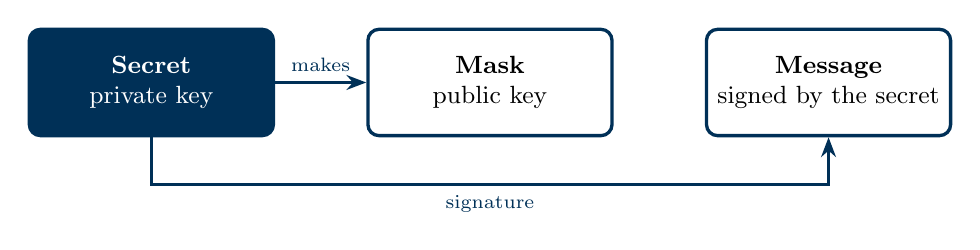
\begin{tikzpicture}[b/.style={draw=gtnavy, very thick, rounded corners, minimum width=3.1cm, minimum height=1.35cm, align=center, font=\small}, a/.style={-{Stealth[length=2.5mm]}, very thick, gtnavy}]
\node[b, fill=gtnavy, text=white] (s) at (0,0) {\textbf{Secret}\\ private key};
\node[b] (m) at (4.3,0) {\textbf{Mask}\\ public key};
\node[b] (g) at (8.6,0) {\textbf{Message}\\ signed by the secret};
\draw[a] (s) -- node[above, font=\scriptsize] {makes} (m);
\draw[a] (s.south) |- ++(0,-0.6) -| node[pos=0.25, below, font=\scriptsize] {signature} (g.south);
\end{tikzpicture}
\end{center}
You are a \textbf{private key}, a secret number as random as a camera filming lava lamps, wearing a mask everyone sees: your \textbf{public key}.
\vspace{2mm}

\textbf{\textcolor{gtnavy}{The magic}}: any observer can prove that the one \textbf{behind} the mask wrote the message, even without ever seeing behind the mask.
\vfill
{\scriptsize Cloudflare makes random numbers by filming a wall of lava lamps (Cloudflare, 2017). This week, a firm browsers trust to vouch for websites was found using the number 4 as a private key.}
\par\vspace{0pt plus 1fill}\hfill{\scriptsize \hyperlink{main-metaphor}{\beamerreturnbutton{Back}}}
\end{frame}


\begin{frame}[label=appx-key]
\frametitle{Whoever Holds the Private Key Controls the Coins}
\lead{Identity. How do I send money in a way no one else can fake?}

\bi
\m Each owner holds a secret \textbf{private key}, and signs payments with it
\m A key is a large random number. Even the best known shortcut to finding one would take the whole Bitcoin network about 11 billion years
\m An AI agent can hold a key, so it can hold and spend money directly
\m The ledger cannot tell the owner from a thief or an AI agent. Math protects the key, but an ordinary burglar can take that key by ordinary force
\ei
\vfill
{\scriptsize Best known attack on a Bitcoin key: about $2^{128}$ steps, counted at the network's pace of 977 million trillion guesses per second (CoinWarz, September 29, 2026). Blind guessing would take about $2^{255}$.}
\par\vspace{0pt plus 1fill}\hfill{\scriptsize \hyperlink{main-metaphor}{\beamerreturnbutton{Back}}}
\end{frame}


\begin{frame}[label=appx-sigformal]
\frametitle{A Digital Signature Proves the Key Holder Sent the Payment}

\begin{columns}[c]
\column{0.46\textwidth}
\centering
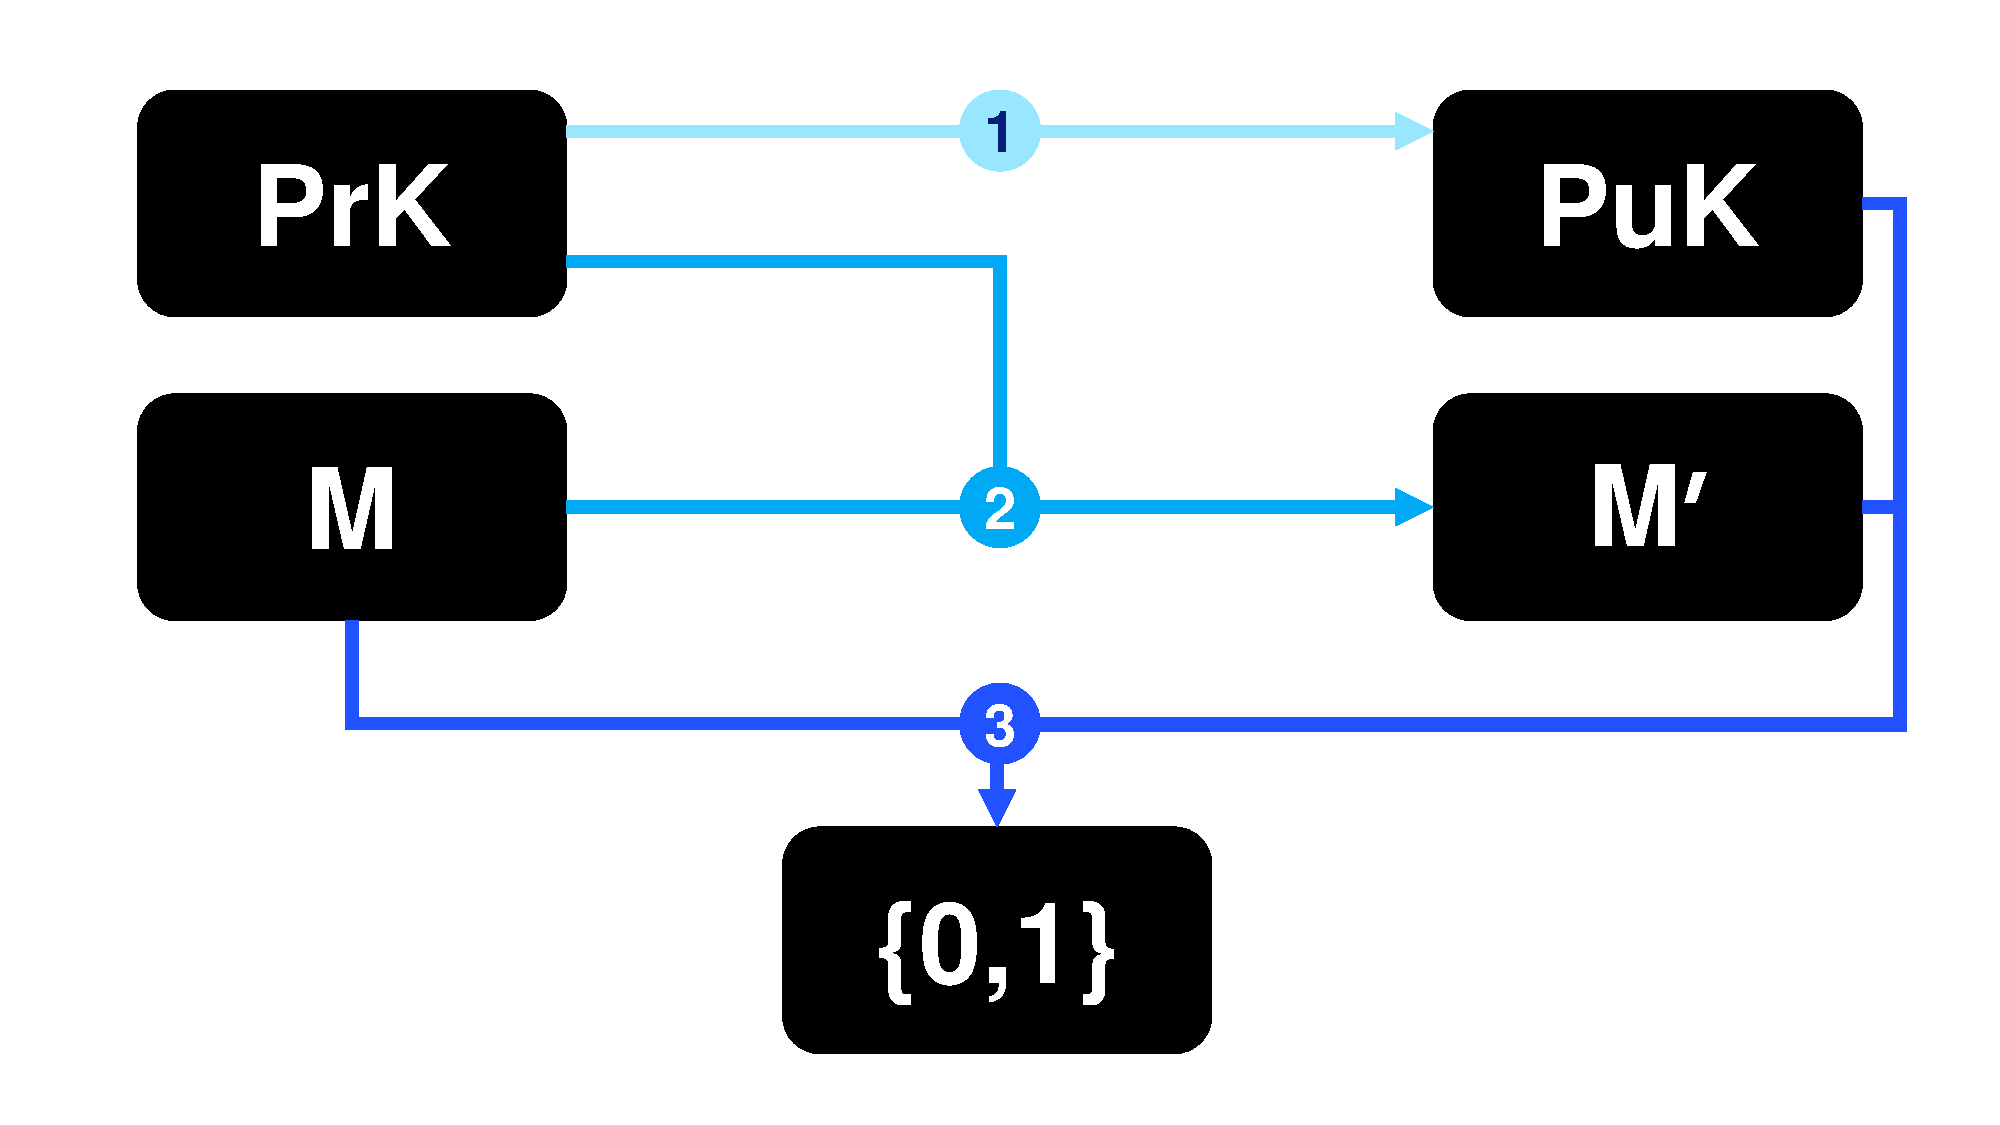
\includegraphics[width=\textwidth]{fig_signature_flow.pdf}\\[1mm]
{\scriptsize PrK private key; PuK public key; M message, such as ``send 1 bitcoin to Brian''; M$'$ signed message; \{0,1\} invalid or valid}
\column{0.52\textwidth}
\small
\be
\m The private key produces the public key, which everyone sees. Working back to the private key is infeasible
\m The private key signs the message. Only the key holder can produce that signature
\m Anyone checks the signature with the public key, and never sees the private key
\ee
\end{columns}
\vspace{3mm}
{\small An agent's payments carry the same proof, so another agent can check them before it deals.}
\par\vspace{0pt plus 1fill}\hfill{\scriptsize \hyperlink{main-metaphor}{\beamerreturnbutton{Back}}}
\end{frame}


\begin{frame}[label=appx-cyberweek]
\frametitle{This Week, Attackers Went After Keys, Wallets and Websites}

\footnotesize
\bi
\m \textbf{Guessable keys (October 17).} eMudhra's eight weak keys were whole numbers from 4 to 237. Each could sign a fake certificate for any website. Browsers blocked them by October 20
\m \textbf{Weak randomness (October 17--18).} The Qubic web wallet made its seeds with Math.random, a generator never meant for secrets. An attacker drained 1,404 wallets in about 100 minutes
\m \textbf{Tampered wallets (October 13--15).} Some Ledger and Trezor wallets from resellers carried implants that leaked the seed phrase or preset it. About \$100 million was stolen
\m \textbf{AI agents (reported October 19).} One hacker's autonomous AI agents probed more than 1,200 websites and broke into about 100 companies, including Deere, SharkNinja and Cummins, for about \$5,000 of AI usage
\m \textbf{Critical PHP flaws (October 21).} Two flaws in PHP, which runs 69\% of websites whose server language is known, let attackers run their own code on web servers. Finland and the Netherlands took government websites offline
\ei
{\small In the key and wallet cases the signature math held. The keys were guessable or stolen.}
\vfill
{\scriptsize Helme; The Register; SlowMist via Crypto Briefing; Zetter, \emph{Zero Day} (Bitquery estimate); php.net; W3Techs; NOS; Valtori; Reuters via The Hacker News. October 13 to 22, 2026.}
\par\vspace{0pt plus 1fill}\hfill{\scriptsize \hyperlink{main-metaphor}{\beamerreturnbutton{Back}}}
\end{frame}


\begin{frame}[label=appx-mandate]
\frametitle{A Signed Mandate Caps What an Agent Can Spend}

\bi
\m Ask an agent to buy golf clubs from Costco for no more than \$600. Google's protocol records a signed ``mandate''
\m If you later deny the purchase, the signature shows what you authorized. The cap holds even if the model misbehaves
\m The code must survive a trial by fire. In simulation, AI agents exploited 51\% of 405 previously hacked contracts (Anthropic, 2025)
\ei
\par\vspace{0pt plus 1fill}\hfill{\scriptsize \hyperlink{main-experiment}{\beamerreturnbutton{Back}}}
\end{frame}


\begin{frame}[label=appx-synthesis]
\frametitle{AI Can Remove the Middleman That Stalled Crypto}

\begin{center}
\small
\begin{tabular}{p{0.2\textwidth} p{0.34\textwidth} p{0.34\textwidth}}
\toprule
 & \textbf{Strength} & \textbf{Weakness} \\
\midrule
AI & Flexible judgment & Hard to hold to exact limits \\
Blockchain & Rules that execute exactly & Complex and hard to use \\
Together & Agents inside limits they cannot rewrite & Buggy code, bad data, and force remain \\
\bottomrule
\end{tabular}
\end{center}

\bi
\m AI is a natural candidate to cut out the middleman and democratize crypto to unsophisticated people. That could be good, disastrous, or overhyped
\ei
\par\vspace{0pt plus 1fill}\hfill{\scriptsize \hyperlink{main-northstar}{\beamerreturnbutton{Back}}}
\end{frame}


\begin{frame}[label=appx-personhood]
\frametitle{Proving Who Stands Behind a Request Remains an Open Problem}

\bi
\m \textbf{Proof of personhood} shows that a person stands behind a key. \textbf{Provenance} records whether a person or an agent made a request, such as an online order
\m Any source of data you give to a computer could be faked, including an AI rendering of a face
\m World reports about 18 million people verified as human in 160 countries (April 2026)
\m Google's Pixel 10 attaches a signed record of how each photo was made at the moment of capture (C2PA, September 2025)
\ei
\par\vspace{0pt plus 1fill}\hfill{\scriptsize \hyperlink{main-northstar}{\beamerreturnbutton{Back}}}
\end{frame}

\begin{frame}[label=appx-switchoff]
\frametitle{For Both Technologies the Board Asks Who Can Switch It Off}

\begin{center}
\begin{tabular}{p{0.27\textwidth} p{0.3\textwidth} p{0.3\textwidth}}
\toprule
 & \textbf{Public blockchain} & \textbf{Enterprise AI} \\
\midrule
Who holds the key & Whoever holds the private key & Whoever holds the model weights \\
Who keeps the record & Thousands of independent validators & The cloud provider \\
Who writes the rules & Contract code & The vendor's terms \\
Who can switch it off & No one & The provider, or its government \\
\bottomrule
\end{tabular}
\end{center}

\par\vspace{0pt plus 1fill}\hfill{\scriptsize \hyperlink{main-northstar}{\beamerreturnbutton{Back}}}
\end{frame}

\begin{frame}[label=appx-sources]
\frametitle{Sources}

\small
\bi
\m Nakamoto (2008); Merkle, U.S. Patent 4,309,569 (1979); Buterin (2013); Lessig (1999); Porter (1979), ``How Competitive Forces Shape Strategy''; Mart\'{i}nez (2022), ``How Much Should We Trust the Dictator's GDP Growth Estimates?''; Huang \& Hall (2026)
\m Anthropic (2025); Google (2025); Coinbase; Circle; JPMorgan; x402.org; World (2026); Tether (BDO); Congressional Research Service; FXC Intelligence; Cambridge (2025); IEA (2025); Energy Institute (2025); Synergy Research; World Nuclear Association; Coin Dance; CoinWarz; Blockchain.com; Yahoo Finance
\m Stablecoins carried 0.31\% of cross-border retail payments in 2025 (FXC Intelligence). In 2024 a new giant data center opened about every 2.7 days (Synergy Research)
\ei
\par\vspace{0pt plus 1fill}\hfill{\scriptsize \hyperlink{main-credits}{\beamerreturnbutton{Back}}}
\end{frame}

\end{document}
